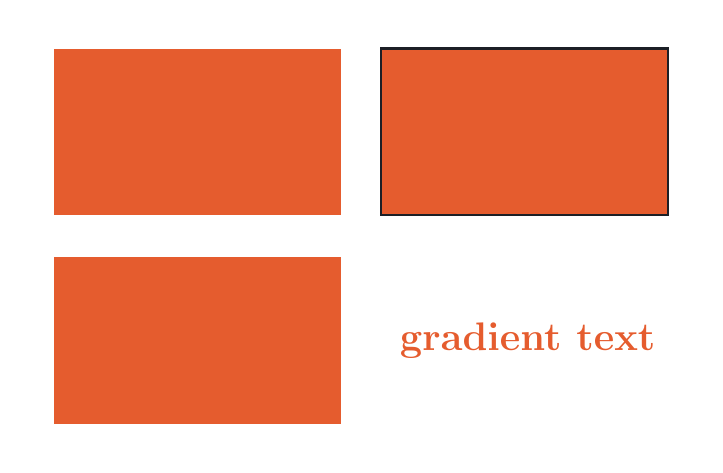
\begin{tikzpicture}[every node/.style={inner sep=0bp,outer sep=0bp}]
  \definecolor{qcA}{rgb}{0.9,0.36,0.18}
  \definecolor{qcB}{rgb}{0.11,0.12,0.15}
  \useasboundingbox (0bp,0bp) rectangle (240bp,150bp);
  \path[fill=qcA] (9.6bp,82.5bp) -- (112.8bp,82.5bp) -- (112.8bp,142.5bp) -- (9.6bp,142.5bp) -- cycle;
  \path[fill=qcA,draw=qcB,line width=0.75bp] (127.2bp,82.5bp) -- (230.4bp,82.5bp) -- (230.4bp,142.5bp) -- (127.2bp,142.5bp) -- cycle;
  \path[fill=qcA] (9.6bp,7.5bp) -- (112.8bp,7.5bp) -- (112.8bp,67.5bp) -- (9.6bp,67.5bp) -- cycle;
  \node[anchor=center,text=qcA,font=\bfseries\fontsize{14}{16.8}\selectfont] at (180bp,37.5bp) {gradient text};
\end{tikzpicture}
